\documentclass[12pt,a4paper]{article}

\usepackage[utf8]{inputenc}
\usepackage[T1]{fontenc}
\usepackage[french]{babel}
\usepackage{graphicx}
\usepackage{hyperref}
\usepackage{geometry}
\geometry{margin=2.5cm}
\usepackage{tikz}
\usetikzlibrary{arrows.meta, positioning, shapes.geometric}

\title{ETL Foot World Cup (1930--2022) \\ \large Rapport de synthèse}
\author{Alexandre Laugier \\ Florian Abgrall \\ Alassane Ndao}
\date{Avril 2026}

\begin{document}

\maketitle
\tableofcontents
\newpage

% ---------------------------------------------------------
\section{Introduction}

Ce rapport présente la construction d'un pipeline ETL complet permettant de centraliser, nettoyer, transformer et charger dans MySQL l'ensemble des matchs de Coupe du Monde FIFA entre 1930 et 2022.  
L'objectif final est de produire un dataset propre et harmonisé, conforme au brief, et d'en extraire quelques KPI pertinents.

\newpage
% ---------------------------------------------------------
\section{Sources de données}

Les données proviennent de plusieurs formats :

\begin{itemize}
    \item CSV historiques (1930--2010)
    \item CSV officiels FIFA 2014
    \item JSON FIFA 2018
    \item JSON officiel 2022
\end{itemize}

\subsection*{Problèmes rencontrés}

\begin{itemize}
    \item incohérences dans les noms d'équipes (accents, variantes, renommages)
    \item incohérences dans les noms de villes
    \item dates dans des formats différents
    \item colonnes manquantes selon les éditions
\end{itemize}

\subsection*{Stratégies de nettoyage}

\begin{itemize}
    \item normalisation Unicode
    \item suppression des espaces superflus
    \item harmonisation des noms via un dictionnaire de correspondance
    \item fusion progressive des datasets nettoyés
\end{itemize}

\newpage
% ---------------------------------------------------------
\section{Pipeline ETL}

Le pipeline ETL principal a été implémenté en Python et s’appuie sur trois scripts principaux, orchestrés par \texttt{main.py} :

\begin{itemize}
    \item \texttt{extract.py} : lecture des fichiers bruts (CSV, JSON), normalisation des colonnes, gestion des encodages et des types ;
    \item \texttt{transform.py} : nettoyage des données (noms d’équipes, villes, stades), harmonisation des formats de dates, fusion des différentes éditions en un dataset unique ;
    \item \texttt{load\_mysql.py} : création des tables si nécessaire, chargement du dataset final dans MySQL, gestion des connexions et des erreurs.
\end{itemize}

La configuration (paramètres de connexion, chemins de fichiers, mappings) est centralisée dans des fichiers YAML sous \texttt{config/}, et les exécutions du pipeline sont tracées dans un fichier de log (\texttt{logs/etl.log}, non versionné).

\paragraph{Rôle du script \texttt{main.py}.}

Le script \texttt{main.py} joue le rôle d’orchestrateur du pipeline ETL.  
Il exécute les trois étapes dans l’ordre logique suivant :

\begin{enumerate}
    \item \textbf{Extraction} via \texttt{extract.py} ;
    \item \textbf{Transformation} via \texttt{transform.py} ;
    \item \textbf{Chargement} via \texttt{load\_mysql.py}.
\end{enumerate}

Cette orchestration garantit que :

\begin{itemize}
    \item chaque étape ne démarre que si la précédente s’est déroulée correctement ;
    \item les erreurs sont capturées et consignées dans le fichier de log ;
    \item le pipeline peut être relancé facilement en une seule commande.
\end{itemize}

Cette structure modulaire rend le pipeline robuste, lisible et facile à maintenir.

Le pipeline ETL Python repose sur une architecture simple et modulaire.  
Chaque étape est isolée dans un script dédié, ce qui facilite la maintenance, la lisibilité et la réutilisation.  
Le schéma ci-dessous illustre le flux général du traitement, depuis les fichiers bruts jusqu’au chargement final dans MySQL.
\begin{figure}[htbp]
    \centering
    \begin{tikzpicture}[
    node distance=2.5cm,
    block/.style={
        rectangle,
        draw,
        rounded corners,
        minimum width=4cm,
        minimum height=1.2cm,
        align=center
    },
    >=stealth
]

\node[block] (extract) {Extraction\\CSV / JSON};
\node[block, right=of extract] (transform) {Transformation\\Nettoyage / Fusion};
\node[block, right=of transform] (load) {Chargement\\MySQL};

\draw[->, thick] (extract.east) -- (transform.west);
\draw[->, thick] (transform.east) -- (load.west);

\end{tikzpicture}

    \caption{Schéma du pipeline ETL Python}
\end{figure}

\subsection*{Intégration de dbt dans le pipeline}

En complément du pipeline ETL Python, une seconde chaîne de traitement a été développée sous \textbf{dbt} afin de valider la cohérence des données et de reconstruire un schéma analytique complet.

L’approche dbt apporte plusieurs avantages :

\begin{itemize}
    \item séparation claire entre \textit{seeds}, \textit{models}, \textit{tests} et \textit{documentation} ;
    \item transformations SQL versionnées et reproductibles ;
    \item génération automatique de documentation ;
    \item possibilité de tester les relations entre dimensions et faits.
\end{itemize}

Les modèles dbt produits par Florian Abgrall et Alassane Ndao ont permis de :

\begin{itemize}
    \item reconstruire les dimensions (\texttt{team}, \texttt{stadium}, \texttt{edition}) ;
    \item générer la table de faits \texttt{fct\_match} ;
    \item vérifier la cohérence des clés étrangères ;
    \item comparer les résultats avec ceux du pipeline Python.
\end{itemize}

Cette double approche (Python + dbt) renforce la robustesse du projet et garantit la qualité du dataset final.
\newpage
% ---------------------------------------------------------
\section{Modélisation des données}

\subsection{Modèle Conceptuel de Données (MCD)}

Le Modèle Conceptuel de Données (MCD) présente les entités principales manipulées dans le projet ainsi que leurs relations.  
Il sert de base à la construction du schéma logique et garantit une vision claire et cohérente du domaine métier.
\begin{figure}[htbp]
    \centering
    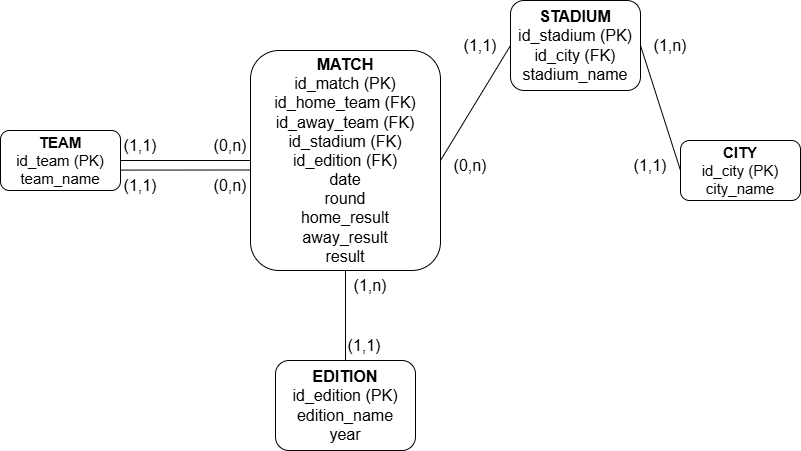
\includegraphics[width=0.9\textwidth]{images/MCD_data_worldcup_foot_1930_2022.drawio.png}
    \caption{Modèle Conceptuel de Données}
\end{figure}

\paragraph{Lecture des cardinalités.}

Le MCD utilise la notation classique (min, max) pour exprimer les cardinalités entre entités :

\begin{itemize}
    \item \textbf{(1,1)} : participation obligatoire et unique ;
    \item \textbf{(0,n)} : participation facultative, avec un nombre potentiellement illimité d’occurrences ;
    \item \textbf{(1,n)} : participation obligatoire, avec au moins une occurrence.
\end{itemize}

Dans notre modèle :

\begin{itemize}
    \item une \textbf{équipe} peut apparaître dans \textbf{0 à n matchs} en tant qu’équipe à domicile ou à l’extérieur ;
    \item un \textbf{match} est associé à \textbf{exactement une équipe à domicile} et \textbf{une équipe à l’extérieur} ;
    \item un \textbf{stade} peut accueillir \textbf{0 à n matchs}, mais chaque match se déroule dans \textbf{un seul stade} ;
    \item une \textbf{édition} contient \textbf{1 à n matchs}, mais chaque match appartient à \textbf{une seule édition}.
\end{itemize}

Cette structure garantit la cohérence du modèle et permet de représenter fidèlement l’organisation des Coupes du Monde.

\newpage

\subsection{Modèle Logique de Données (MLD)}

Le Modèle Logique de Données (MLD) traduit le MCD en structures relationnelles concrètes.  
Il définit les clés primaires, les clés étrangères et les types de données utilisés dans la base MySQL.
\begin{figure}[htbp]
    \centering
    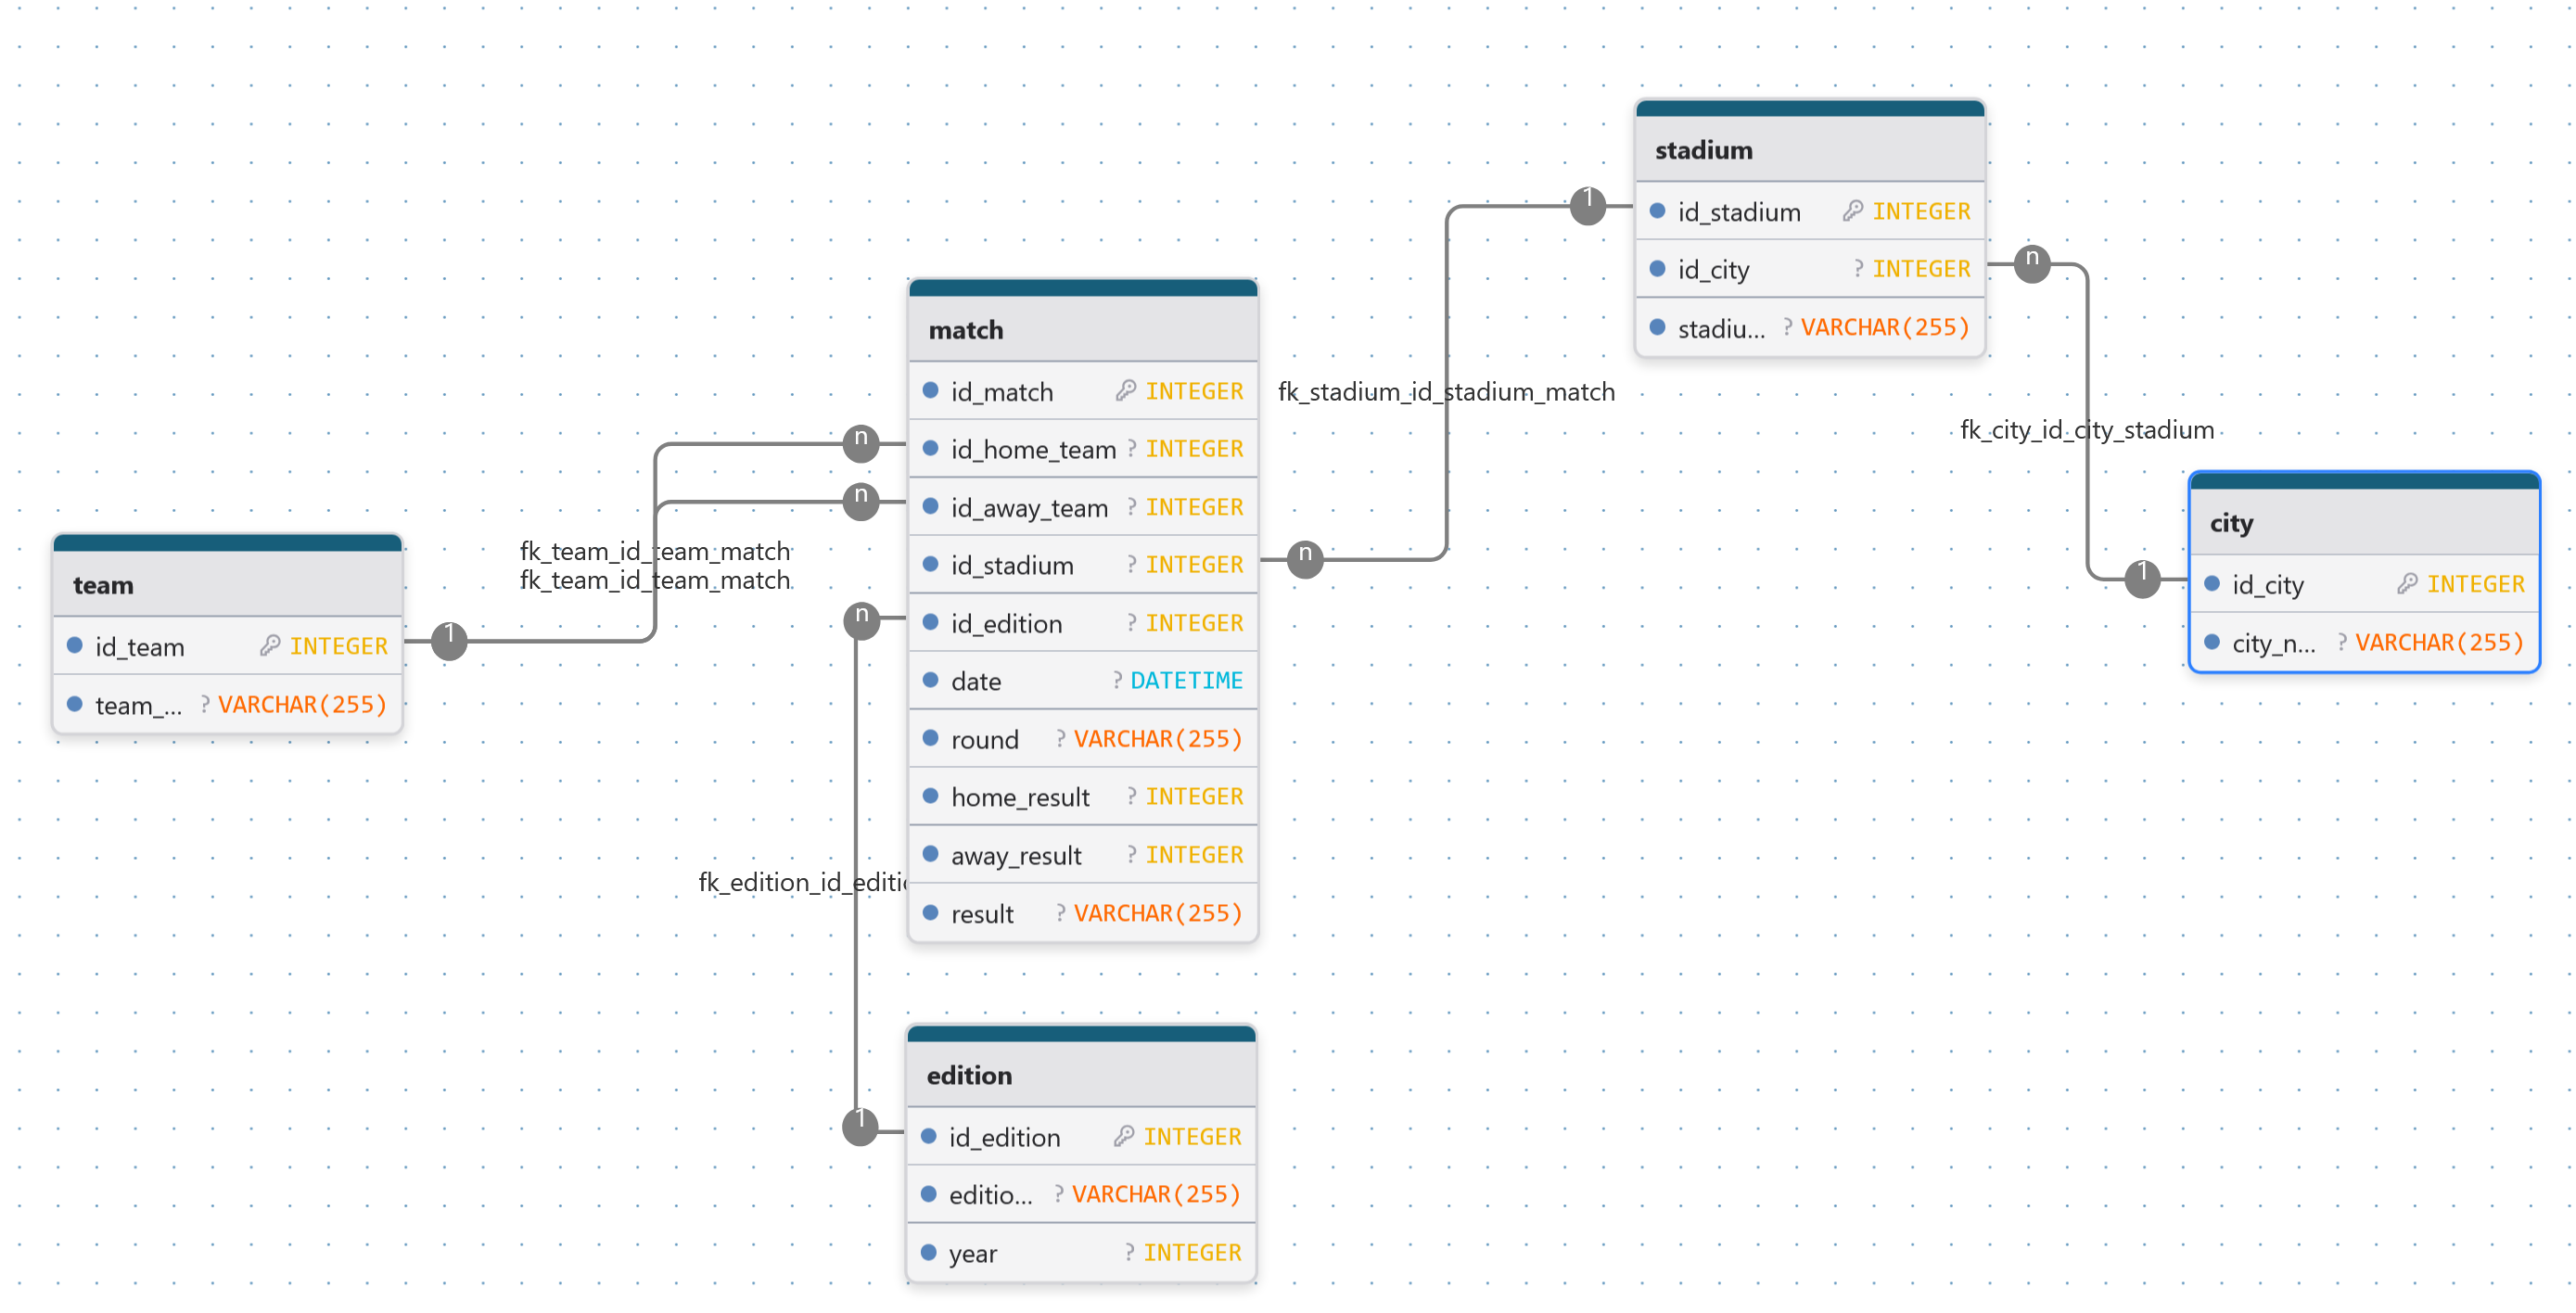
\includegraphics[width=\textwidth]{images/MLD_data_worldcup_foot_1930_2022.png}
    \caption{Modèle Logique de Données}
\end{figure}

\paragraph{Clés primaires et clés étrangères.}

Dans le MLD, chaque table possède une clé primaire (\textbf{PK}) permettant d’identifier de manière unique chaque enregistrement.  
Ces clés sont définies comme des entiers auto-incrémentés dans MySQL, ce qui garantit :

\begin{itemize}
    \item l’unicité des identifiants ;
    \item la simplicité des jointures ;
    \item la stabilité des clés même en cas de modifications des données sources.
\end{itemize}

Les clés étrangères (\textbf{FK}) assurent la cohérence référentielle entre les tables :

\begin{itemize}
    \item \texttt{match.id\_home\_team} et \texttt{id\_away\_team} référencent \texttt{team.id\_team} ;
    \item \texttt{match.id\_stadium} référence \texttt{stadium.id\_stadium} ;
    \item \texttt{match.id\_edition} référence \texttt{edition.id\_edition}.
\end{itemize}

Ces contraintes garantissent que :

\begin{itemize}
    \item aucun match ne peut exister sans équipes valides ;
    \item aucun match ne peut référencer un stade inexistant ;
    \item chaque match appartient à une édition valide.
\end{itemize}

L’ensemble de ces règles assure l’intégrité du schéma relationnel et la fiabilité des analyses réalisées à partir de la base.

\newpage
% ---------------------------------------------------------
\section{Chargement MySQL}

Le chargement des données dans MySQL constitue la dernière étape du pipeline ETL Python.  
Il est assuré par le script \texttt{load\_mysql.py}, qui :

\begin{itemize}
    \item établit la connexion à MySQL via les paramètres définis dans \texttt{config/db\_config.yaml} ;
    \item crée les tables si elles n'existent pas encore (DDL) ;
    \item applique les contraintes d'intégrité (clés primaires, clés étrangères) ;
    \item insère les données nettoyées et harmonisées dans les tables cibles ;
    \item journalise chaque opération dans le fichier de log.
\end{itemize}

Le schéma SQL complet est disponible dans \texttt{sql/schema.sql}.  
Il définit les tables suivantes :

\begin{itemize}
    \item \texttt{team} : dimension des équipes ;
    \item \texttt{city} : dimension des villes ;
    \item \texttt{stadium} : dimension des stades ;
    \item \texttt{edition} : dimension des éditions de Coupe du Monde ;
    \item \texttt{match} : table de faits contenant l’ensemble des matchs.
\end{itemize}

\paragraph{Vue analytique.}

En complément des tables physiques, une vue \texttt{match\_final} a été créée afin de faciliter les analyses.  
Elle combine les informations des dimensions (\texttt{team}, \texttt{stadium}, \texttt{edition}) avec la table de faits \texttt{match}.  
Cette vue sert de base à l’ensemble des KPI et permet d’interroger directement un dataset propre et harmonisé.

Des vérifications d’intégrité supplémentaires sont regroupées dans \texttt{sql/quality\_checks.sql}, notamment :

\begin{itemize}
    \item détection de doublons ;
    \item vérification des clés étrangères ;
    \item contrôle de cohérence des dates et des scores.
\end{itemize}

\newpage
% ---------------------------------------------------------
\section{KPI}

Les indicateurs clés (KPI) sont calculés à partir de la table finale \texttt{match\_final}.  
Ils permettent d’analyser l’évolution du football international sur près d’un siècle.

Les principaux KPI produits sont :

\begin{itemize}
    \item \textbf{Nombre de matchs par édition} : mesure l’évolution du format de la compétition ;
    \item \textbf{Total de buts par édition} : permet d’identifier les éditions les plus offensives ;
    \item \textbf{Moyenne de buts par match} : indicateur global de performance offensive ;
    \item \textbf{Équipes les plus victorieuses} : classement basé sur les résultats cumulés ;
    \item \textbf{Scores les plus fréquents} : analyse des tendances de résultats.
\end{itemize}

Les requêtes SQL correspondantes sont regroupées dans \texttt{sql/queries\_kpi.sql}.  
Elles ont été exécutées dans MySQL et leurs résultats ont été vérifiés pour garantir la cohérence du dataset final.

\paragraph{Exemples de requêtes SQL.}

Voici quelques exemples de requêtes utilisées pour produire les KPI :

\begin{itemize}
    \item \textbf{Nombre de matchs par édition}
\begin{verbatim}
SELECT edition_name, COUNT(*) AS nb_matchs
FROM match_final
GROUP BY edition_name
ORDER BY edition_name;
\end{verbatim}

    \item \textbf{Moyenne de buts par match}
\begin{verbatim}
SELECT AVG(home_result + away_result) AS avg_goals
FROM match_final;
\end{verbatim}

    \item \textbf{Équipes les plus victorieuses}
\begin{verbatim}
SELECT t.team_name, COUNT(*) AS wins
FROM match_final m
JOIN team t ON t.id_team = m.id_home_team
WHERE m.result = 'home'
GROUP BY t.team_name
ORDER BY wins DESC;
\end{verbatim}

\end{itemize}

Ces requêtes sont regroupées dans \texttt{sql/queries\_kpi.sql} et ont été exécutées dans MySQL pour produire les indicateurs présentés.

\newpage
% ---------------------------------------------------------
\section{Travail collaboratif}

Ce projet a été réalisé en trinôme avec \textbf{Florian Abgrall} et \textbf{Alassane Ndao}.  
La collaboration a été essentielle pour couvrir l’ensemble des aspects du pipeline ETL et de la modélisation analytique.

\subsection*{Contribution de Florian Abgrall (dbt)}

Florian a pris en charge la construction d’un \textbf{modèle analytique complet sous dbt}, permettant de reconstruire un schéma en étoile à partir des données nettoyées.  
Son travail inclut notamment :

\begin{itemize}
    \item la configuration du projet dbt (\texttt{dbt\_project.yml}) ;
    \item la définition des seeds (\texttt{seeds/schema.yml}) pour les datasets bruts ;
    \item la création des dimensions :
    \begin{itemize}
        \item \texttt{dim\_team.sql} : extraction et normalisation de tous les noms d’équipes ;
        \item \texttt{dim\_stadium.sql} : harmonisation des stades ;
        \item \texttt{dim\_edition.sql} : gestion des éditions de Coupe du Monde.
    \end{itemize}
    \item la construction de la table de faits \texttt{fct\_match.sql}, intégrant :
    \begin{itemize}
        \item les résultats des matchs ;
        \item les clés étrangères vers les dimensions ;
        \item la normalisation des rounds ;
        \item la fusion des éditions 1930--2010, 2014 et 2022.
    \end{itemize}
\end{itemize}

Ce travail dbt a permis de valider la cohérence du schéma en étoile et de comparer les résultats avec le pipeline ETL Python.

\subsection*{Contribution d'Alassane Ndao}

Alassane a contribué à plusieurs étapes clés :

\begin{itemize}
    \item nettoyage initial des données 1930--2010 ;
    \item exploration des incohérences dans les noms d’équipes et de stades ;
    \item participation à la construction des dimensions dbt ;
    \item relecture et validation des transformations ;
    \item tests croisés entre dbt et l’ETL Python.
\end{itemize}

\subsection*{Synthèse}

Le travail collaboratif a permis :

\begin{itemize}
    \item de croiser deux approches complémentaires : ETL Python et modélisation dbt ;
    \item de valider la qualité des données via deux pipelines indépendants ;
    \item d’obtenir un schéma analytique robuste et cohérent ;
    \item de renforcer la fiabilité des KPI produits.
\end{itemize}

\newpage
% ---------------------------------------------------------
\section{Conclusion}

Ce projet a permis de construire un pipeline ETL complet et robuste couvrant près d’un siècle de données de Coupe du Monde.  
L’approche adoptée — extraction, transformation, puis chargement dans MySQL — a permis d’obtenir un dataset propre, harmonisé et conforme aux exigences du brief.

Le travail réalisé met en évidence plusieurs points forts :

\begin{itemize}
    \item une architecture Python modulaire, facilitant la maintenance et l’évolution du pipeline ;
    \item un nettoyage approfondi des données, indispensable compte tenu de l’hétérogénéité des formats et des incohérences historiques ;
    \item une modélisation relationnelle cohérente, appuyée par un MCD et un MLD solides ;
    \item une vue analytique \texttt{match\_final} permettant d’interroger facilement les données consolidées ;
    \item une validation croisée grâce à une seconde chaîne de traitement sous dbt, renforçant la fiabilité du schéma en étoile ;
    \item la production de KPI pertinents permettant d’analyser l’évolution du football international sur près d’un siècle.
\end{itemize}

Le travail collaboratif avec Florian Abgrall et Alassane Ndao a été un atout majeur, permettant de confronter deux approches complémentaires (Python et dbt) et d’assurer une qualité optimale du dataset final.

Plusieurs pistes d’amélioration pourraient être envisagées :

\begin{itemize}
    \item automatisation complète du pipeline via un orchestrateur (Airflow, Prefect) ;
    \item ajout de visualisations avancées (heatmaps, timelines, analyses par continent) ;
    \item intégration d’éditions futures pour maintenir le dataset à jour ;
    \item déploiement du modèle dbt sur un entrepôt cloud pour faciliter la scalabilité.
\end{itemize}

Ce projet constitue ainsi une base solide pour des analyses plus poussées, des visualisations enrichies ou une industrialisation complète du traitement des données sportives.

\end{document}
